The performance of the FVR method is shown theoretically in this section. The size of the volumes being registered is defined as $N^3$ and each frame is sampled at a resolution of $W$ $\times$ $H$. The projection process requires $12WH$ operations whilst re-sampling the point cloud requires $2WH$ operations. The Volume Registration process, $VolumeRegister{\theta \varphi t_x t_y t_z}(V_1, V_2)$ consists of 2 $\times$ Hanning windowing processes, 2 $\times$ 3D FFTs, 2 $\times$ volume-logs, 2 $\times$ log-spherical transforms, 2 $\times$ phase correlation processes and 1 $\times$ linear transformation and peak finding. 

The Hanning windowing function requires 26 operations. The 3D FFT has complexity of $3N^3\log{N}$, the log and log-spherical transform functions require 3 and 58 operations per voxel respectively. Multiplying two frequency spectra together and transforming a volume requires 15 and 30 operations per voxel respectively. Finding the peak value requires $2N^3$ operations. The complexity in terms of number of operations for the phase correlation process is given in Eq. \ref{eqn:PCFULLPERFORMANCE} This process requires 2 $\times$ 3D FFTs, 1 $\times$ frequency spectra multiplication, and 1 $\times$ peak finding operation. 
\begin{equation} \label{eqn:PCFULLPERFORMANCE}
6N^3\log{N} + 2N^3 + 15
\end{equation}
The total complexity can then be found by taking into account the projection and re-sampling totals as well as the total for $VolumeRegister{\theta \varphi t_x t_y t_z}(V_1, V_2)$. Tallying the number of operations for each process and multiplying them by number of times the process is performed gives us the number of operations as a function of $W$, $H$ and $N$ in Eq. \ref{eqn:FULLPERFORMANCE}.
\begin{equation} \label{eqn:FULLPERFORMANCE}
6N^3 + 28WH + 18(N^3\log{N}) + 230
\end{equation}


To compare performance of the generic volume registration method with the speed up, we use the complexity defined in equation \ref{eqn:FULLPERFORMANCE}. Here, we ignore the cost of projecting the depth map. The 3D DFT has complexity $3N^3log(N)$. This is the first step (see figure \ref{fig:PIPELINE3}), the next is the spherical-map transform which is complexity $45N^3$. If processed on the GPU the performance becomes 45 operations per voxel assuming that one voxel is assigned to one unit of processing. A 3D transform is 30 operations per voxel, 2D phase correlation requires 15 operations to multiply the frequency spectra and $2N^2log(N)$ operations to do the 2D FFT. Finally a projection map transform requires 1 operation per voxel. \\

In total, the proposed method requires $2 \times$ 3D FFTs, $2 \times$ spherical-map transforms, $1 \times$ 3D geometrical transformation, $3 \times$ 2D phase correlations and $4 \times$ projection map transforms. The total complexity is added up for all of these functions and given in equation \ref{eqn:FULLPERF2}. \\

\begin{equation} \label{eqn:FULLPERF2}
6log(N)\times (N^3 + N^2) + 169
\end{equation}

Figure \ref{fig:perfComp} provides a visualization of the performance improvement which the proposed method achieves over the original Fourier volume registration approach. It is clear that the proposed method is around 3 times faster
than the original Fourier based volume registration approach. This is due to the reduction in the amount of data to process afforded by the novel spherical-map transform and orthogonal projection methods.

\begin{figure}[t]
\centering
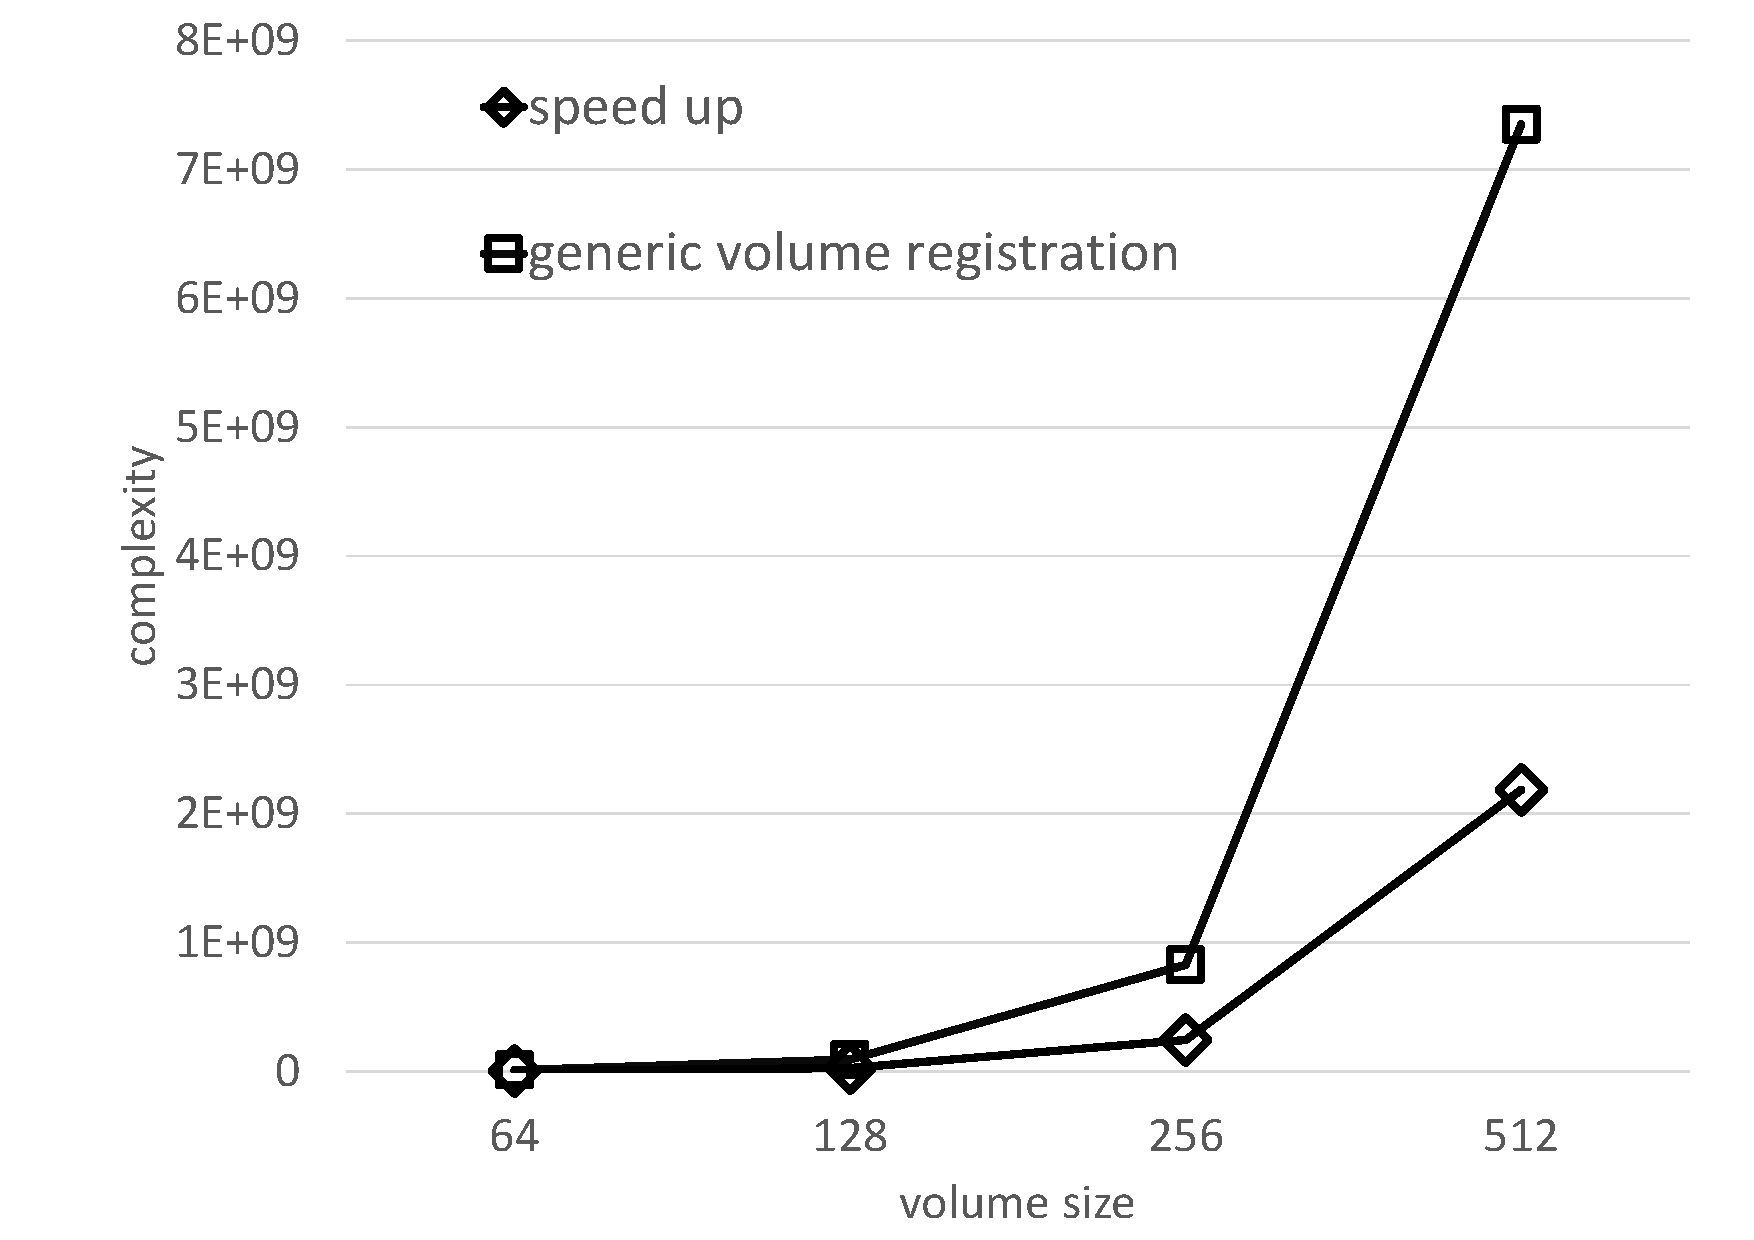
\includegraphics[width=3.0in]{images/results/performance/comparison}
\caption{Comparison of performance between volume registration and the proposed speed up for different volume sizes.}
\label{fig:perfComp}
\end{figure}